\glsreset{ntu-rgbd}
\Gls{ntu-rgbd} is a large-scale dataset for human activity analysis. It contains over 56 thousand video samples and 4 million frames. The NTU RGB+D dataset contains 60 action classes such as drinking, eating, staggering, punching and kicking \autocite{Shahroudy_2016_CVPR}. 

The dataset is collected using Microsoft Kinect v2 sensors, in which they collected four modalities: depth maps, 3D joint information, RGB frames and IR sequences. In total, 25 body joints were captured in the dataset, in which each body joint is represented by x-coordinates, y-coordinates and depth \autocite{Shahroudy_2016_CVPR}. The body joints are illustrated in \cref{fig:ntu_body_joints}. 

\begin{figure}[!ht]
    \centering
    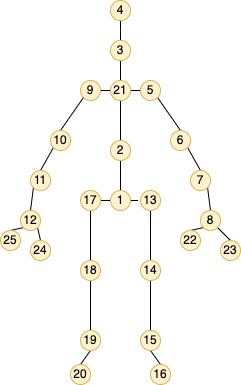
\includegraphics[width=5cm]{figures/nturgb.drawio.png}
    \caption{1-base of the spine, 2-middle of the spine; 3-neck, 4-head, 5-left shoulder, 6-left elbow, 7-left wrist, 8-left hand, 9-right shoulder, 10-right elbow, 11-right wrist, 12-right hand, 13-left hip, 14-left knee, 15-left ankle, 16-left foot, 17-right hip, 18-right knee, 19-right ankle, 20-right foot, 21-spine, 22-tip of the left hand, 23-left thumb, 24-tip of the right hand, 25-right thumb}
    \label{fig:ntu_body_joints}
\end{figure}

The NTU RGB+D dataset was later expanded into a new one named NTU RGB+D 120. The new dataset contains 114 480 video samples of 120 action classes, all from 106 separate human subjects. 

The NTU RGB+D dataset has been employed in numerous studies, making it a well-established choice for research in the field of \gls{HAR} \autocite{yan2018spatial, si2019attention, cheng2020skeleton}. The dataset's large scale and diverse range of activities facilitate the training of models with high generalisation capabilities, which aligns with the goals of this study in achieving optimal final validation accuracy. Given the dataset's widespread application and success in \gls{HAR}-related research, it is an appropriate foundation for this investigation.